%%
%% ****** ljmsamp.tex 13.06.2018 ******
%%
\documentclass[
11pt,%
tightenlines,%
twoside,%
onecolumn,%
nofloats,%
nobibnotes,%
nofootinbib,%
superscriptaddress,%
noshowpacs,%
centertags]%
{revtex4}
\usepackage{ljm}
\usepackage{listings}
\usepackage{amsmath,amsthm,amscd,amsfonts,amssymb}
\usepackage{textcomp}
\usepackage{graphicx}
\usepackage{esvect}
\usepackage{physics}

\lstset{
language=C++,
basewidth=0.5em,
xleftmargin=45pt,
xrightmargin=45pt,
basicstyle=\small\ttfamily,
keywordstyle=\bfseries\underbar,
numbers=left,
numberstyle=\tiny,
stepnumber=1,
numbersep=10pt,
showspaces=false,
showstringspaces=false,
showtabs=false,
frame=trBL,
tabsize=2,
captionpos=t,
breaklines=true,
breakatwhitespace=false,
escapeinside={\%*}{*)}
}

\begin{document}

\titlerunning{Деформирование поверхностной сетки в двумерном случае} % for running heads
\authorrunning{A.~A.~Rybakov and S.~S.~Shumilin} % for running heads
%\authorrunning{First-Author, Second-Author} % for running heads

\title{Сравнение приближенных методов деформирования поверхностной сетки в двумерном случае}
% Splitting into lines is performed by the command \\
% The title is written in accordance with the rules of capitalization.

\author{\firstname{A.~A.}~\surname{Rybakov}}
\email[E-mail: ]{rybakov.aax@gmail.com} \affiliation{Joint
Supercomputer Center of the Russian Academy of Sciences (JSCC RAS)
-- Branch of Scientific Research Institute of System Analysis of the
Russian Academy of Sciences, Leninsky prospect 32a, Moscow, 119334,
Russia}

\author{\firstname{S.~S.}~\surname{Shumilin}}
\email[E-mail: ]{shumilin@jscc.ru} \affiliation{Joint Supercomputer
Center of the Russian Academy of Sciences (JSCC RAS) -- Branch of
Scientific Research Institute of System Analysis of the Russian
Academy of Sciences, Leninsky prospect 32a, Moscow, 119334, Russia}
%\noaffiliation % If the author does not specify a place of work.

\firstcollaboration{(Submitted by TODO : SUBMITTER)} % Add if you know submitter.
%\lastcollaboration{ }

\received{TODO : DATE} % The date of receipt to the editor, i.e. December 06, 2017

\begin{abstract}
Численное моделирование процесса обледенения поверхности включает в себя работу разных решателей, выполняющихся итерационно и обменивающихся между собой расчетными данными.
Цепочка выполнения расчетов состоит из работы газодинамического решателя, расчета жидкой фазы, вычисления толщины ледяного нароста на поверхностной сетке и перестроения поверхности.
После выполнения перестроения поверхности процесс моделирования уходит на следующую итерацию в газодинамический решатель.
Таким образом выполнение качественного перестроения поверхностной расчетной сетки с учетом наросшего льда влияет на все дальнейшие вычисления.
В статье рассмотрены приближенные методы перестроения поверхностной сетки по данным нароста льда в каждой ячейке для двумерного случая и оценена их точность.
\end{abstract}

\subclass{TODO : CODE} % Enter 2010 Mathematics Subject Classification.

\keywords{TODO : KEYWORDS} % Include keywords separeted by comma.

\maketitle

% Text of article starts here.

\section{Introduction}

Задача расчета обледенения аэродинамических поверхностей является крайне актуальной на сегодняшний день.
Из наиболее известных программных продуктов, реализующих данный функционал, можно прежде всего выделить такие пакеты как FENSAP-ICE \cite{Bourgault_FENSAP}, LEWICE \cite{Bidwell_LEWICE}, CANICE \cite{Pueyo_CANICE}, CHT2D \cite{Pueyo_CHT2D} и многие другие.
Как правило эти пакеты являются многошаговыми и предусматривают итерационное перестроение поверхностной сетки по мере нарастания льда.
Такое перестроение требуется выполнять, так как по мере нарастания льда необходимо повторно запускать аэродинамический решатель для получения актульных данных о движении среды вокруг нового деформированного тела \cite{Ozgen, Beaugendre}.
Для получения более точного профиля ледяного нароста требуется производить перестроение поверхностной сетки как можно чаще, поэтому скорость работы алгоритмов перестроения сетки также существенна.

Наиболее острый интерес представляет разработка алгоритмов перестроения поверхностных сеток в трехмерном пространстве.
Среди таких можно отметить алгоритм перестроения с локальным сохранением объема ячеек \cite{Jiao}, нашедший свою реализацию в инструменте iceSurf \cite{Thompson}.
Однако работы по разработке алгоритмов перестроения поверхностей в двумерном пространстве также ведутся, и результаты данных исследований в той или иной мере переносятся на работу в трехмерное пространство, как это продемонстрировано в работе \cite{Pueyo}.

В данной работе проанализированы приближенные методы перестроения поверхностной сетки только для двумерного случая, однако они могут быть обобщены и на трехмерные объекты.
В дальнейшем задача перестроения поверхностной сетки рассматривается в абстрактном виде без привязки к проблематике обледенения поверхностей.

\section{Решение задачи о перестроении поверхности в двумерном пространстве}

Рассмотрим геометрическую задачу о перестроении поверхности в двумерном пространстве в общем виде.
Пусть даны $n$ ячеек поверхностной сетки, каждая из которых представлена отрезком длины $l_i$ (то есть общее количество узлов равно $n + 1$).
Известно направление изменения поверхности каждой ячейки (направление нормали к отрезку), а также направление движения каждого узла $\overline{g_i}$, $|\overline{g_i}| = 1$.
Оно совпадает с направлением суммы единичных нормалей, проведенных к инцидентным ячейкам.
К тому же для двумерного случая данное направление лежит на биссектрисе угла, образованного двумя инцидентными ячейками \cite{Fortin} (Fig.~\ref{fig:grid_normals}).

\begin{figure}[h]
\setcaptionmargin{5mm}
\onelinecaptionstrue
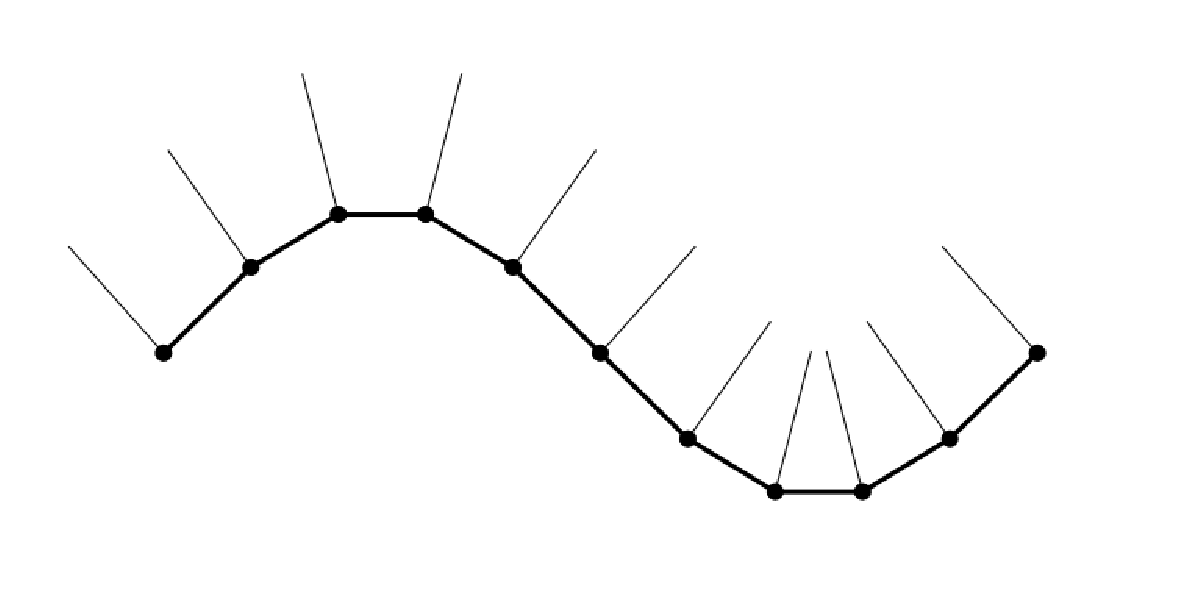
\includegraphics[width=0.8\textwidth]{pics/grid_normals.pdf}
\captionstyle{normal}\caption{Поверхностная сетка с обозначенными направлениями движения узлов.}
\label{fig:grid_normals}
\end{figure}

Также известны локальные сдвиги поверхности для каждой ячейки (они задаются значениями $H_i$).
Требуется найти такие значения локальных сдвигов узлов сетки $h_i$, чтобы охватывающая площадь между старой поверхностью и новой поверхностью для каждой ячейки сетки ($S_i$) как можно меньше отличалась от требуемого значения $T_i = l_iH_i$.

Для решения данной задачи сначала требуется вычислить охватывающую площадь для каждой отдельной ячейки.

\subsection{Задача о вычислении охватывающей площади при движении узлов отдельной ячейки}

Рассматривается ячейка, представленная на плоскости отрезком $AB$ длины $l$.
При перемещении точек $A$ и $B$ в новые точки $A_1$ и $B_1$ соответственно образуется четырехугольник $AA_1B_1B$.
Требуется найти его площадь, выраженную явно через параметры $a = \overline{AA_1}$ и $b = \overline{BB_1}$ (Fig.~\ref{fig:local}).

\begin{figure}[h]
\setcaptionmargin{5mm}
\onelinecaptionstrue
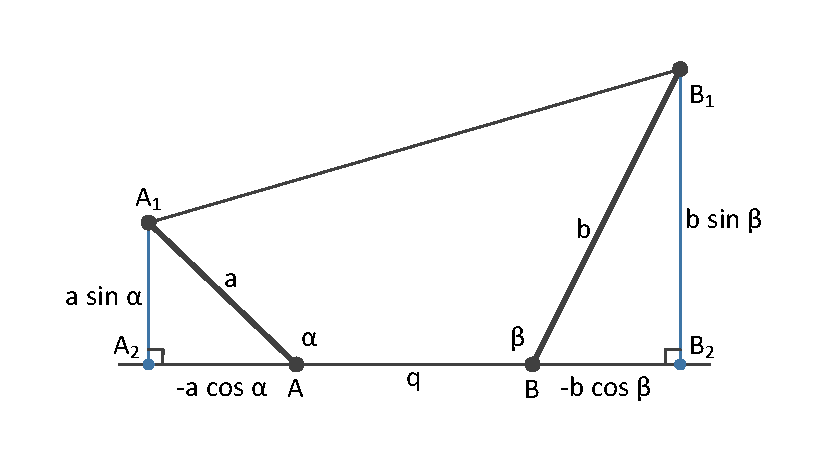
\includegraphics[width=0.8\textwidth]{pics/local.pdf}
\captionstyle{normal}\caption{Вычисление охватывающей площади при передвижении узлов ячейки.}
\label{fig:local}
\end{figure}

Для решения задачи опустим перпендикуляры из точек $A_1$ и $B_1$ на прямую $AB$.
Их основаниями будут точки $A_2$ и $B_2$ соответственно.
Искомая площадь может быть представлена в следующем виде:

\begin{equation}
S_{AA_1B_1B} = S_{A_2A_1B_1B_2} - S_{AA_1A_2} - S_{BB_1B_2}
\end{equation}

Обозначим угол между векторами $\overline{AA_1}$ и $\overline{AB}$ через $\alpha$, а угол между векторами $\overline{BB_1}$ и $\overline{BA}$ через $\beta$.
Тогда искомая площадь вычисляется явно в следующем виде:

\begin{equation}
S_{AA_1B_1B} = \frac{1}{2}(l - a \cos \alpha - b \cos \beta)(a \sin \alpha + b \sin \beta) + \frac{1}{2}a^2 \sin \alpha \cos \alpha + \frac{1}{2}b^2 \sin \beta \cos \beta
\end{equation}

\begin{equation}
S_{AA_1B_1B} = \frac{1}{2}\big(l(a \sin \alpha + b \sin \beta) - ab \sin(\alpha + \beta)\big)
\end{equation}

\subsection{Решение методом градиентного спуска}

Метод градиентного спуска является одним из наиболее простых методом оптимизации для нахождения локального минимума функции.
При условии, что в любой точки функции можно вычислить ее градиент, то начиная с некоторого начального приближения $x_0$ строится итерационная последовательность~\cite{Kantorovich}:

\begin{equation}
x^{k+1} = x^k - \gamma _k \nabla f(x_k)
\end{equation}

где $\gamma _k \geq 0$ задает длину шага и, соответственно, скорость градиентного спуска.

Градиентный метод находит свое основное применение в задаче поиска минимума или максимума функции.
Направление антиградиента является направлением наискорейшего убывания функции.
Основная проблема метода заключается в выборе шага $\gamma$.
При больших значениях шага существует вероятность "перепрыгнуть" через минимум функции.
К тому же, метод не гарантирует нахождение глобального минимума.

Рассмотрим решение поставленной задачи методом градиентного спуска.
Неизвестными параметрами являются величины сдвигов узлов сетки $h_i$.
Опираясь на решение локальной задачи об определении охватывающей площади, можно записать охватывающую площадь при движении отдельной ячейки:

\begin{equation}
S_i = \frac{1}{2}\big(l_i(h_i \sin \alpha_i + h_{i + 1} \sin \beta_i) - h_ih_{i + 1} \sin(\alpha_i + \beta_i)\big) 
\end{equation}

Отклонением охватывающей площади в ячейке от истинного значения будем называть величину $\delta_i = S_i - T_i$, а ошибкой -- ее квадрат $d_i = \delta_i^2$.
Общая ошибка при перестроении поверхности задается как сумма ошибок для всех ячеек:

\begin{equation}
D = \sum_{i = 0}^{n - 1}{d_i}
\end{equation}

При нахождении оптимального решения требуется минимизировать общую ошибку.
Для нахождения градиента требуется вычислить частные производные функции $D$ по всем неизвестным $h_i$.
Данные производные можно записать в явном виде.

\begin{equation}
\frac{\partial D}{\partial h_i} = \frac{\partial d_{i - 1}}{\partial h_i} + \frac{\partial d_i}{\partial h_i}
\end{equation}

где

\begin{equation}
\begin{cases}
\frac{\partial d_{i - 1}}{\partial h_i} = \delta_{i - 1}(l_{i - 1} \sin \beta_{i - 1} - h_{i - 1} \sin(\alpha_{i - 1} + \beta_{i - 1})) \\
\frac{\partial d_i}{\partial h_i} = \delta_i(l_i \sin \alpha_i - h_{i + 1} \sin(\alpha_i + \beta_i))
\end{cases}
\end{equation}

Также при осуществлении метода градиентного спуска требуется следить за соблюдением дополнительных условий, которые накладываются на неизвестные $h_i$.
Например, очевидным условием является выполнение соотношения $h_i \ge 0$, что запрещает движение сетки в отрицательном направлении.
В данной работе использовались более строгие условия $min(H_{i - 1}, H_i) \le h_i \le max(H_{i - 1}, H_i)$, которые не позволят величинам смещения узлов сетки выходить за пределы смещений инцидентных им ячеек сетки.

\section{Схемы приближенного решения}

Решение задачи о перестроении сетки методом градиентного спуска оказывается слишком требовательной к ресурсам задачей при увеличении размера сетки.
К тому же качество решения зачастую оказывается неудовлетворительным, особенно при попадании в локальные минимумы.
Поэтому для решения поставленной задачи были предложены методы приближенного решения, основанные на аппроксимации решения в каждой ячейке с помощью примитивных геометрических фигур.

\subsection{Решение методом прямоугольников}

В качестве первого метода рассмотрим приближение, при котором каждый узел сетки сдвигается на вектор $\frac{1}{2}(H_{i - 1} + H_i)\overline{g_i}$.
Данный метод соответствует приближению решения в каждой ячейке прямоугольником по сторонами $l_i$ и $H_i$, а затем усреднения, как показано на Fig.~\ref{fig:grid_rectangles}.

\begin{figure}[h]
\setcaptionmargin{5mm}
\onelinecaptionstrue
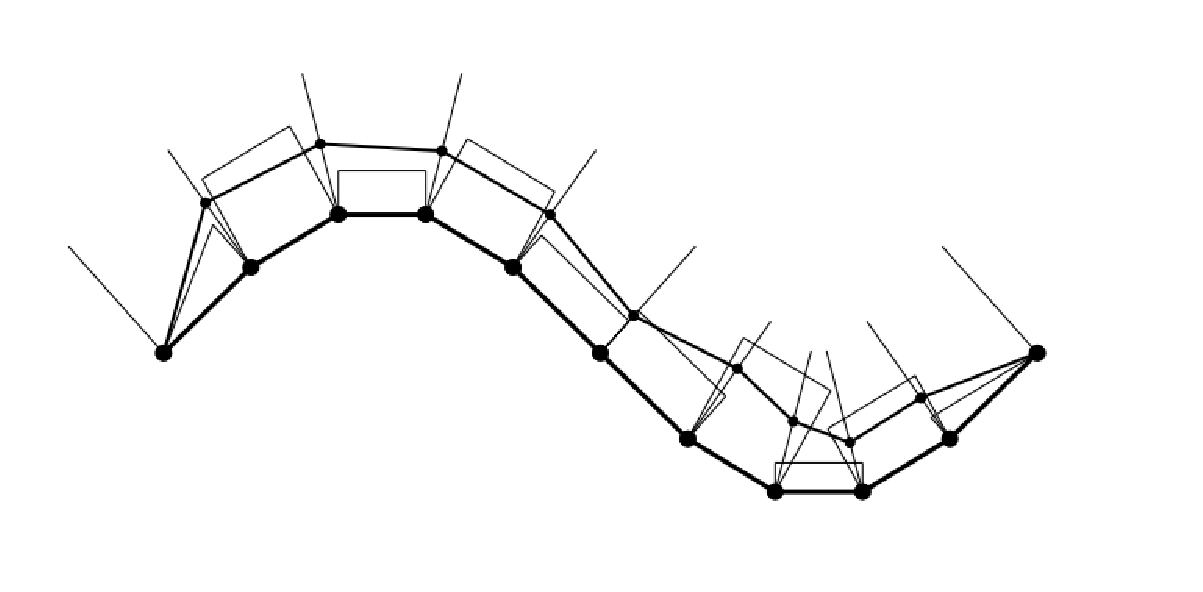
\includegraphics[width=0.8\textwidth]{pics/grid_rectangles.pdf}
\captionstyle{normal}\caption{Перестроение поверхности методом прямоугольников.}
\label{fig:grid_rectangles}
\end{figure}

Стоит отметить возможное развитие данного подхода с помощью применения многослойного приближения, как это описано в работе \cite{Bourgault_Cote}, однако в данной работе эта возможность не рассматривалась.

\subsection{Решение методом трапеций}

В методе трапеций решение в каждой ячейке приближается трапецией с площадью $T_i$, боковые стороны которой лежат на направлениях роста двух узлов, относящихся к рассматриваемой ячейке.
После построения трапеций для всех ячеек сетки у каждого внутреннего узла появляется две новые потенциальные позиции для сдвига (образованные ячейкой слева и ячейкой справа).
В качестве финальной новой позиции выбирается их среднее значение (Fig.~\ref{fig:grid_trapeziums}).

\begin{figure}[h]
\setcaptionmargin{5mm}
\onelinecaptionstrue
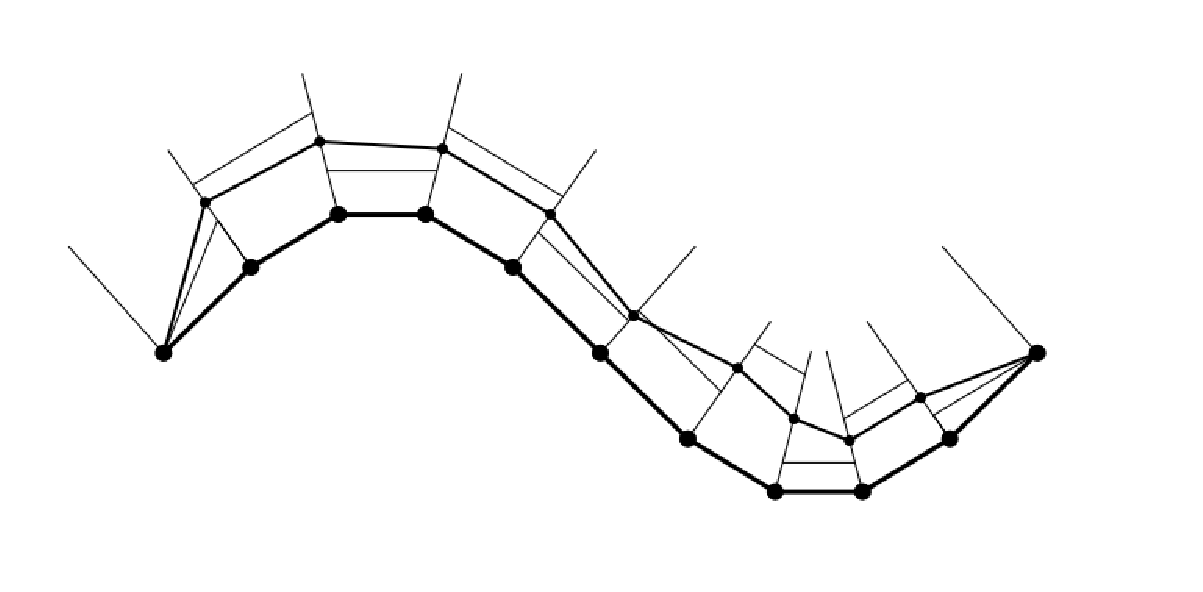
\includegraphics[width=0.8\textwidth]{pics/grid_trapeziums.pdf}
\captionstyle{normal}\caption{Перестроение поверхности методом трапеций.}
\label{fig:grid_trapeziums}
\end{figure}

\subsection{Сравнение точности решений}

Для сравнения точности решений, полученных с помощью описанных методов была использована модельная двумерная поверхностная сетка, представленная одним периодом синусоиды ($x \in [0, 2 \pi]$).
В качестве набора смещений ячеек ($H_i$) использовались одинаковые смещения на величину, равную половине размера ячейки.
При увеличении количества узлов оба приближенных метода продемонстрировали стремление к нулю величины $\frac{D}{\sum_i{T_i}}$ с незначительными отклонениями друг от друга и от метода градиентного спуска, который использовался для верификации.
Также было проведено сравнение величин $\delta_i$ для всех ячеек для предложенных приближенных методов.
Результаты сравнения на модельной сетке при количестве узлов $n = 1000$ приведены на Fig.~\ref{fig:graphic}.

\begin{figure}[h]
\setcaptionmargin{5mm}
\onelinecaptionstrue
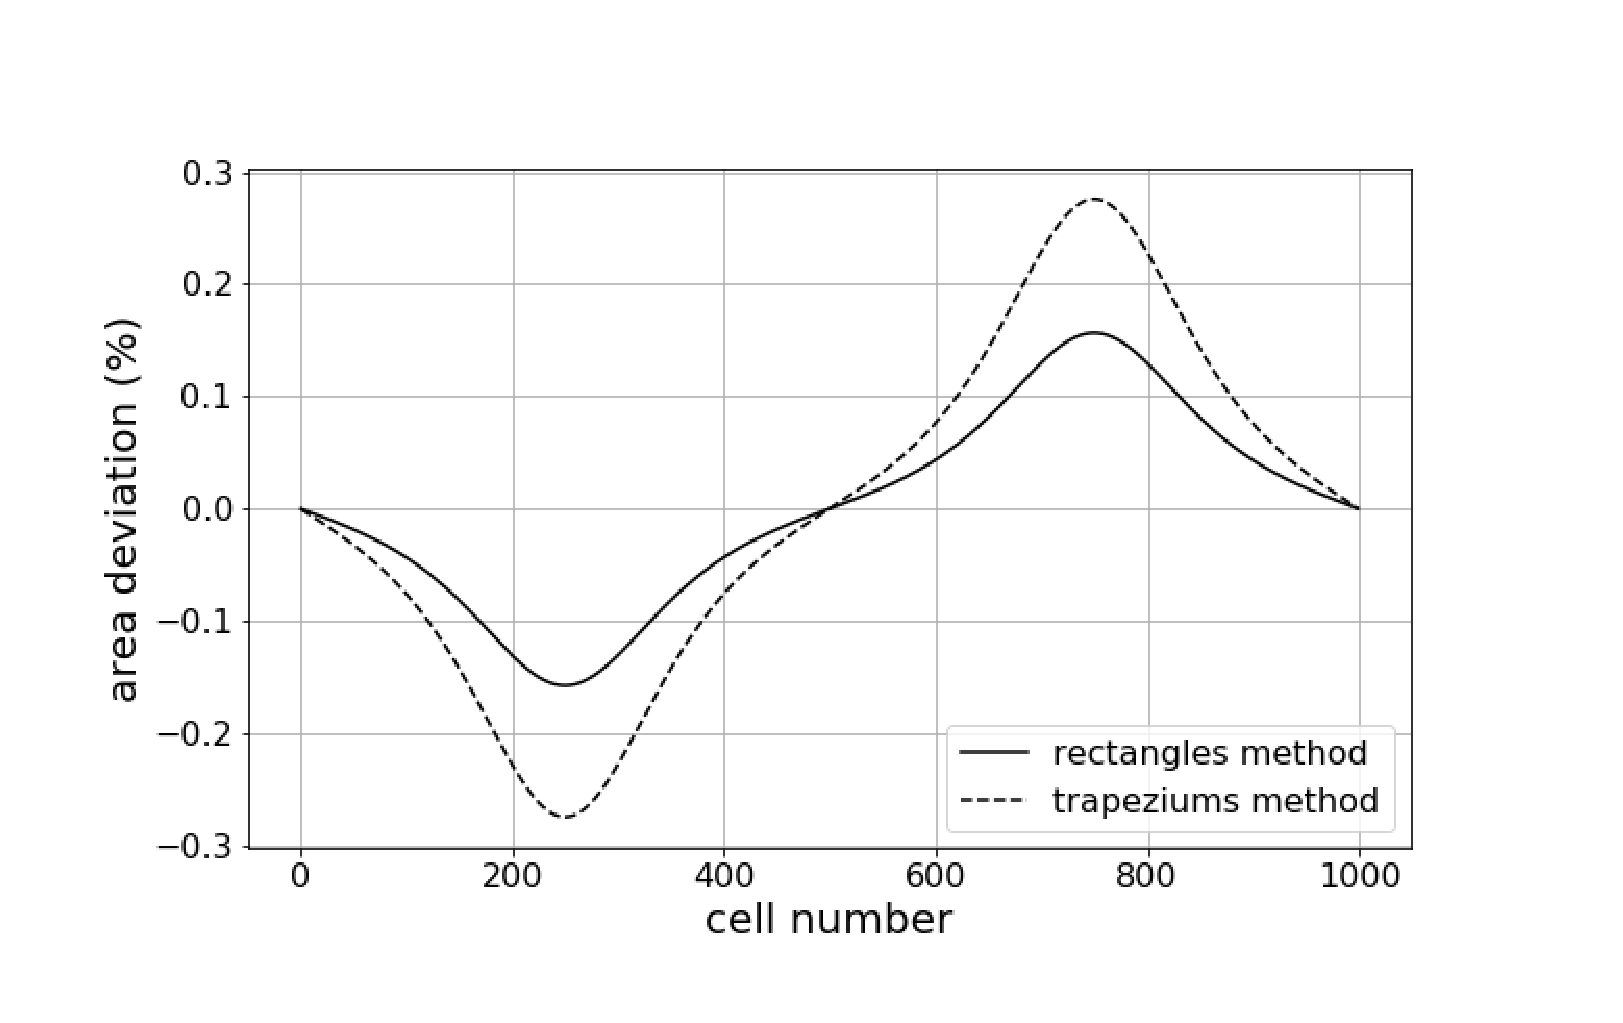
\includegraphics[width=1.0\textwidth]{pics/graphic.pdf}
\captionstyle{normal}\caption{Сравнение точности решений методом прямоугольников и методом трапеций.}
\label{fig:graphic}
\end{figure}

Из данного графика видно, что более простой метод прямоугольников является в то же время и более точным, так как обеспечивает меньшие отклонения от точного решения на сильно выпуклых и сильно вогнутых участках сетки.

\section{Conclusion}

Были рассмотрены два простых приближенных метода перестроения поверхностной сетки в двумерном пространстве.
Сравнение результаты их работы с локально-оптимальным решением, полученным с помощью итерационного метода градиентного спуска показал нецелесообразность использования последнего для промышленного счета.
Из двух приближенных методов перестроения метод прямоугольников продемонстрировал меньшие отклонения решения для отдельных ячеек сетки в местах сильной кривизны сетки.
Рассмотренные приближенные методы могут быть распространены на трехмерный случай, однако это выходит за рамки данной статьи.

\begin{acknowledgments}
The work has been done at the JSCC RAS as part of the state assignment for the topic 0065-2019-0016 (reg. no. AAAA-A19-119011590098-8). The supercomputer MVS-10P, located at the JSCC RAS, was used for calculations during the research.
\end{acknowledgments}

\begin{thebibliography}{99}

\bibitem{Bourgault_FENSAP}
\refitem{article}
Y.~Bourgault, H.~Beaugendre, W.~G.~Habashi, {\it ``Development of a shallow-water icing model in FENSAP-ICE"}, Journal of Aircraft, Vol.~37, No.~4, 640 -- 646 (2000).

\bibitem{Bidwell_LEWICE}
\refitem{article}
C.~Bidwell, D.~Pinella, P.~Garrison, {\it ``Ice accretion calculations for a commercial transport using the LEWICE3D, ICEGRID3D and CMARC programs"}, AIAA Paper 99-0250, Reno (1999).

\bibitem{Pueyo_CANICE}
\refitem{articlce}
A.~Pueyo, D.~Chocron, F.~Kafyeke, {\it ``Improvements to the ice accretion code CANICE"}, CASI $8^{TH}$ Aerodynamics Symposium, Toronto (2001).

\bibitem{Pueyo_CHT2D}
\refitem{article}
A.~Pueyo, D.~Chocron, F.~Mokhtarian, F.~Kafyeke, {\it ``CHT2D: A 2D hot air anti-icing analysis tool"}, $50^{TH}$ Annual General Meeting (AGM) and Conference, Canadian Aeronautics and Space Institute (2003).

\bibitem{Ozgen}
\refitem{article}
S.~\"Ozgen, M.~Canibek, {\it ``Ice accretion simulation on multi-element airfoils using extended Messinger model"}, Heat Mass Transfer, 45, 305 -- 322 (2009).

\bibitem{Beaugendre}
\refitem{article}
H.~Beaugendre, {\it ``A PDE-based 3D approach to in-flight ice accretion"}, PHD Thesis, McGill University, Montreal, QC (2003).

\bibitem{Jiao}
\refitem{article}
J.~Jiao, {\it ``Volume and feature preservation in surface mesh optimization"}, Proceedings, $15^{TH}$ International Meshing Roundtable, Springer-Verlag, Birmingham, AL, 359 -- 374 (2006).

\bibitem{Thompson}
\refitem{article}
D.~Thompson, X.~Tong, Q.~Arnoldus, E.~Collins, D.~McLaurin, E.~Luke, {\it ``Discrete surface evolution and mesh deformation for aircraft icing applications"}, In $5^{TH}$ AIAA Atmospheric and Space Environments Conference. AIAA Paper 2013-2544 (2013).

\bibitem{Pueyo}
\refitem{article}
A.~Pueyo, {\it ``Efficient 3D artificial ice shapes simulations with 2D ice accretion codes using a 3-level correction"}, In SAE 2013 AeroTech Congress and Exhibition, Vol.~7, SAE Technical Paper 2013-01-2136 (2013).

\bibitem{Fortin}
\refitem{article}
G.~Fortin, A.~Ilinca, J.-L.~Laforte, V.~Brandi, {\it ``New roughness computation method and geometric accretion model for airfoil icing"}, Journal of Aircraft, Vol.~41, No.~1, 119-127 (2004).

\bibitem{Kantorovich}
\refitem{book}
G.~P.~Akilov, L.~V.~Kantorovich, {\it ``Functional analysis"}, 2nd ed., Pergamon Press (1982). 

\bibitem{Bourgault_Cote}
\refitem{article}
S.~Bourgault-C\^ot\'e, K.~Hasanzadeh, P.~Lavoie, E.~Laurendeau, {\it ``Multi-layer icing methodologies for conservative ice growth"}, In $7^{TH}$ European Conference for Aeronautics and Aerospace Sciences (EUCASS) (2017).

\end{thebibliography}

\end{document}
